
\documentclass{beamer}
\usepackage[utf8]{inputenc}
\usepackage[ngerman]{babel}
\usepackage{multicol}
\usepackage[utf8]{inputenc}
\usepackage[T1]{fontenc}
\usepackage[ngerman]{babel}
\usepackage{amsmath}
\usepackage{amsfonts}
\usepackage{amssymb}
%\usepackage{paralist}
\usepackage{color}
\usepackage{xcolor}
\usepackage{lmodern}
\usepackage{graphicx}
\usepackage[mediumspace,mediumqspace,squaren]{SIunits} %SI-Einheiten
\usepackage[version=3]{mhchem} %chemische Formeln
\usepackage{tabularx, calc} %Tabellen
\usepackage{multirow} %Tabelle: mehrere Spalten vereinigen
\usepackage{booktabs} %Verbesserung der Tabellenqualität
\usepackage{caption} %Abbildungs- und Tabellenbeschriftung
\usepackage{array} %Matheumgebung ähnlich tabular
\usepackage{pgf}
\usepackage{dcolumn}
\usepackage{beamerthemeshadow}
\usepackage{comment}
\usepackage{framed}
\usepackage{longtable}
 \usepackage{arydshln}
\beamersetuncovermixins{\opaqueness<1>{25}}{\opaqueness<2->{15}}
\begin{document}
\title{Bachelorarbeit}
\subtitle{Disambiguierungsstrategien in Dialogsystemen }  
%\title{Disambiguierungsstrategien in Dialogsystemen }
%\subtitle{Bachelorarbeit}
\author{Lena Enzweiler}
\institute{Universität des Saarlandes}
\date{\today} 

\beamertemplatenavigationsymbolsempty

\setbeamertemplate{footline}[frame number]

\frame{\titlepage} 

\section{Einleitung}
\subsection{Einleitung}
\frame{\frametitle{Automobile Anwendung}
\begin{figure}[h]
%\caption{Funktionsweise der odp-s3 Platform der Semvox GmbH}
	%\centering
        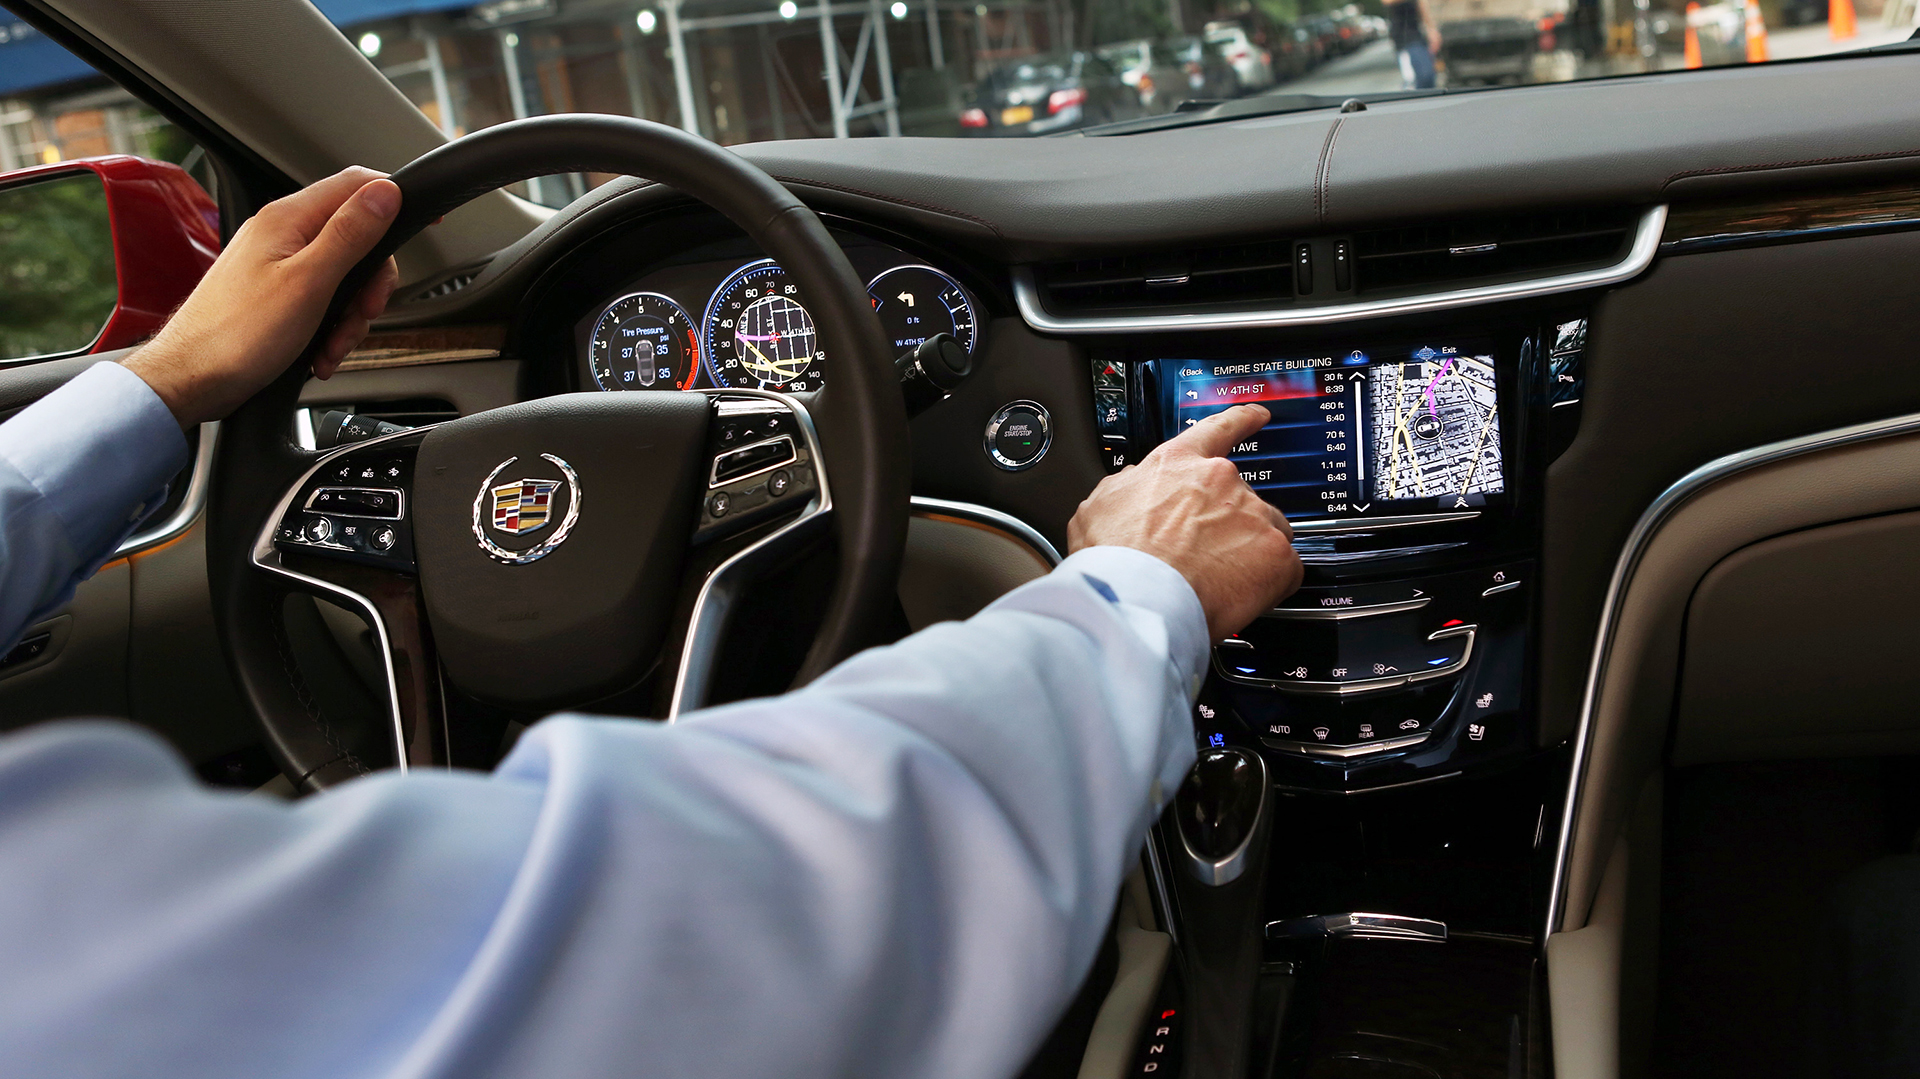
\includegraphics[scale=0.1]{danger}
\end{figure}
\begin{itemize}
	\item Während Autofahrt kognitive Belastung
	\item manuelle Bedienung des Systems zusätzlich belastend
	\item Sprachsteuerung sicherer und weniger belastend. \newline
	Vorrausetzung: durchdachte Dialogsysteme

	
\end{itemize}
}

\subsection{Einleitung}
\frame{\frametitle{Dialogsystem in automobilen Anwendungen}
Effiziente Dialogsysteme im Auto müssen folgende Punkte erfüllen
\begin{figure}[h]
%\caption{Funktionsweise der odp-s3 Platform der Semvox GmbH}
	%\centering
        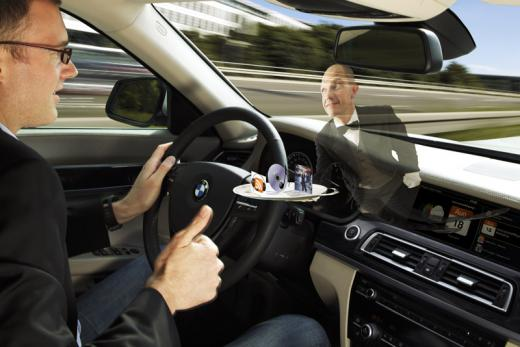
\includegraphics[scale=0.26]{incarassi}
\end{figure}
\begin{itemize}
\item Ablenkung während der Fahrt vermeiden
\item alle Informationen kurz und verständlich übermitteln
\item einfache und intuitive Bedienung garantieren 
\end{itemize} 

$\rightarrow$ Sprachäußerungen müssen raffiniert gestaltet werden
}
\subsection{Einleitung}
\frame{\frametitle{Einleitung}
\begin{figure}[htbp]
	% minipage mit (Blind-)Text
	\begin{minipage}{0.5\textwidth} 
	\begin{itemize}
	\item "Rufe Peter an!"
	\newline
	\pause
	\item System muss über Peter Meier und Peter Müller disambiguieren
	\newline
	\pause
	\item unterschiedliche Disambiguierunsstrategien anwendbar
	\newline
	\end{itemize}
	\end{minipage}
	% Auffüllen des Zwischenraums
	\hfill
	% minipage mit Grafik
	\begin{minipage}{0.45\textwidth}
	% \textwidth bezieht sich nun auf die Minipage
	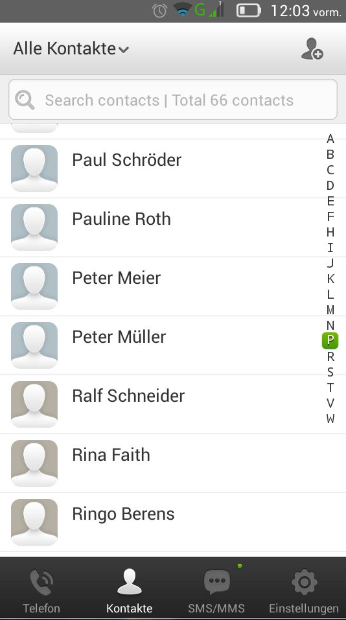
\includegraphics[scale=0.33]{peter}
	\label{Adressbuch} 
	\end{minipage}
% \caption{noch eine Caption}
\end{figure}
\pause
$\rightarrow$ 3 Disambiguierungstrategien untersucht
}


\subsection{Einleitung}
\frame{\frametitle{Einleitung}
\begin{figure}[h]
%\caption{Funktionsweise der odp-s3 Platform der Semvox GmbH}
	%\centering
        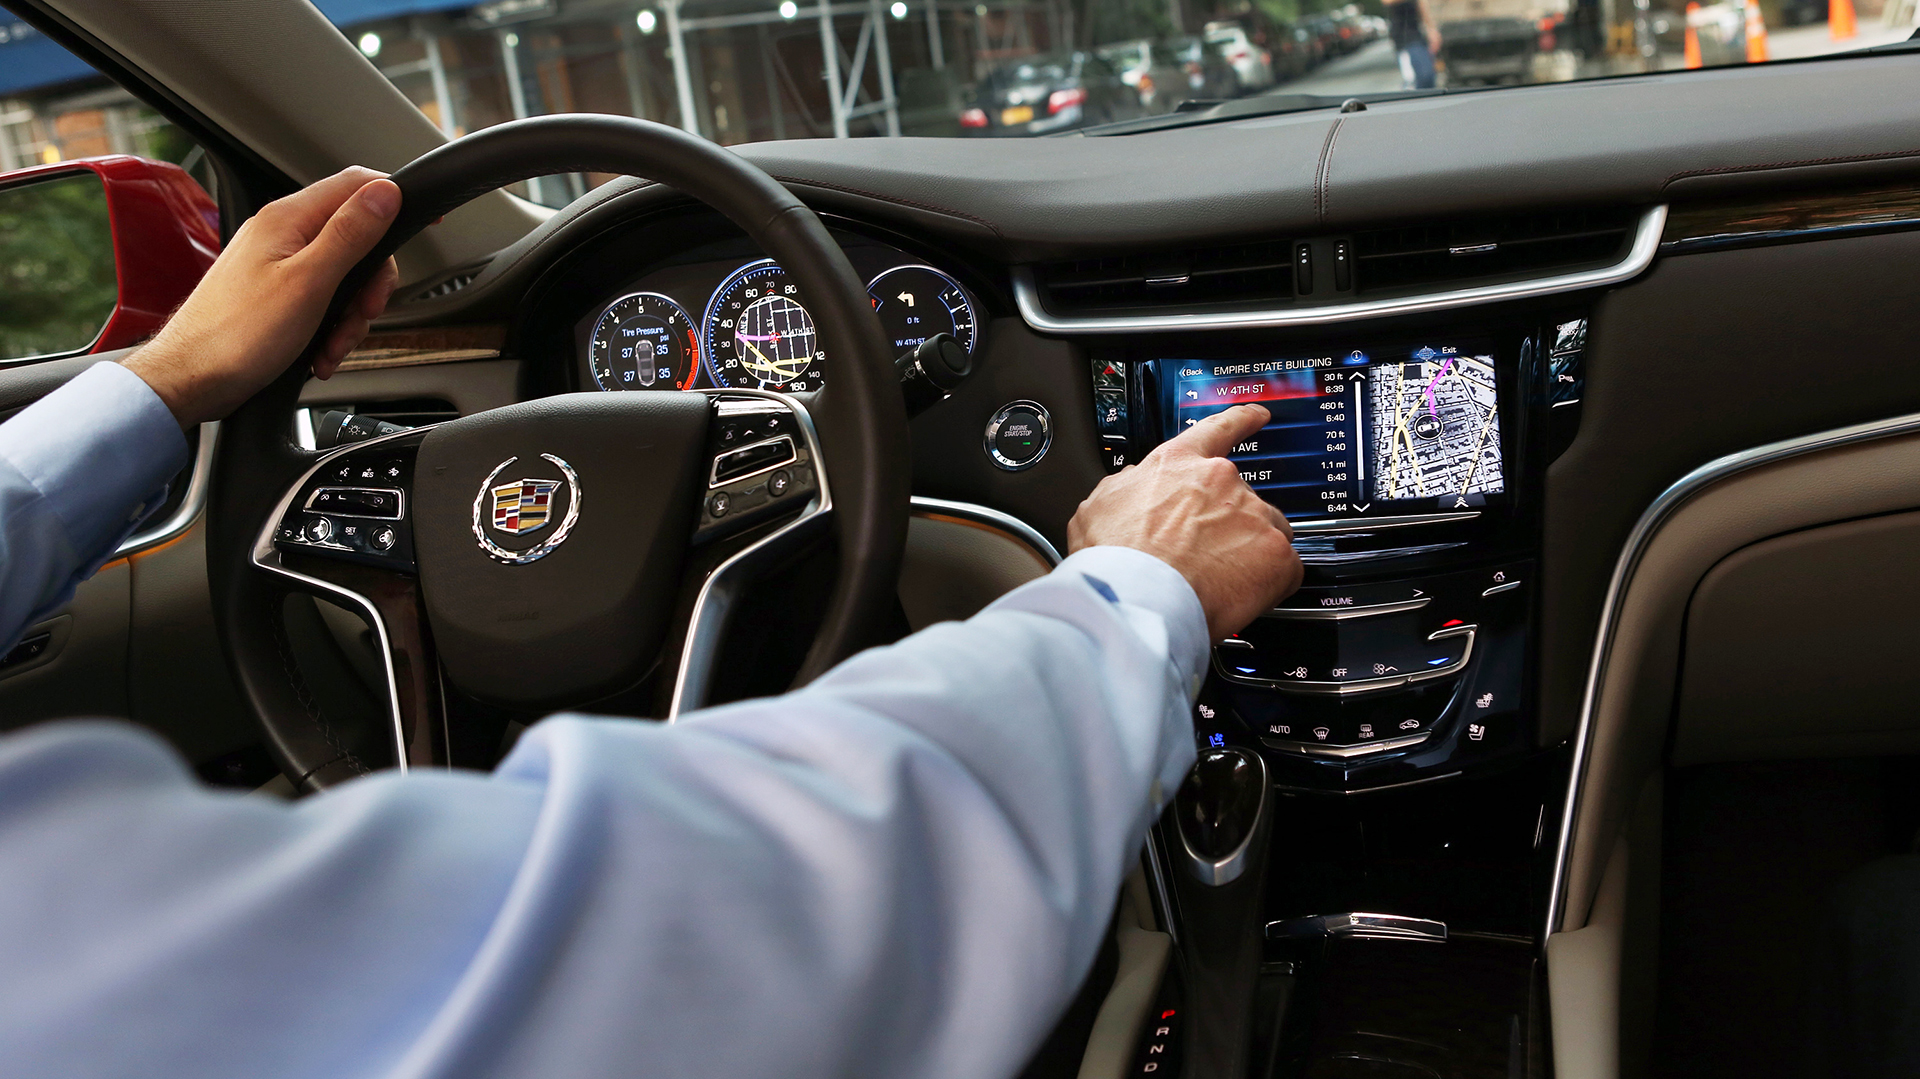
\includegraphics[scale=0.1]{danger}
\end{figure}
\begin{itemize}
	\item Während Autofahrt kognitive Belastung
	\item manuelle Bedienung des Systems zusätzlich belastend
	\item Sprachsteuerung sicherer und weniger belastend. \newline
	Vorrausetzung: durchdachte Dialogsysteme

	
\end{itemize}
}

\subsection{Einleitung}
\frame{\frametitle{Dialogsystem in automobilen Anwendungen}
Effiziente Dialogsysteme im Auto müssen folgende Punkte erfüllen
\begin{figure}[h]
%\caption{Funktionsweise der odp-s3 Platform der Semvox GmbH}
	%\centering
        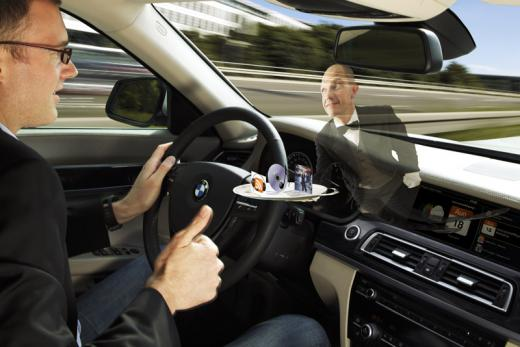
\includegraphics[scale=0.26]{incarassi}
\end{figure}
\begin{itemize}
\item Ablenkung während der Fahrt vermeiden
\item alle Informationen kurz und verständlich übermitteln
\item einfache und intuitive Bedienung garantieren 
\end{itemize} 

$\rightarrow$ Sprachäußerungen müssen raffiniert gestaltet werden
}

\begin{comment}
\subsection{Dialogsysteme}
\frame{\frametitle{Dialogsysteme}
\begin{figure}[h]
\caption{Funktionweise der odp-s3 Platform der Semvox GmbH}
	%\centering
        \fbox{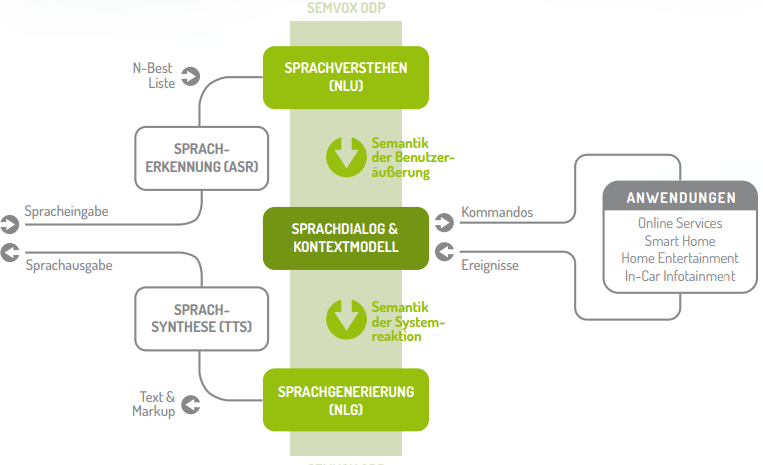
\includegraphics[scale=0.30]{odps3}}
\end{figure}
\begin{itemize}
\item Spracheingabe als semantisches Objekt interpretiert
\item Objekt von Sprachdialog- und Kontextmodell verarbeitet                                                                                                                                                                                                                                                                                                                                                                                                                                                                                                                                                                                                                                                                                                                                                                                                                                                                                                                                                                                                                                                                                                                                                                                                                                                                         
\item Systemreaktion als Sprachausgabe realisiert
\end{itemize} 
}
}
\end{comment}

\subsection{Fokus der Studie}
\frame{\frametitle{Fokus der Studie}
\begin{itemize}
\item ambige Eingaben des Benutzers möglich
\item System muss Mehrdeutigkeit der Eingaben auflösen
\newline
\end{itemize}
$\rightarrow$ Disambiguierung durch geschicktes Nachfragen beim Benutzer
\newline
\newline
%Fokus der Studie:
\begin{block}{Fokus der Studie} Welche Disambiguierungsstrategie eignet sich für Dialogsysteme in einer automobilen Anwendung?  \end{block} 
}
\section{Disambiguierungsstrategien}
\subsection{Disambiguierung}
\frame{\frametitle{Disambiguierung}
Abgrenzung verschiedener Bedeutungen

\begin{figure}[h]
	%\centering
        \fbox{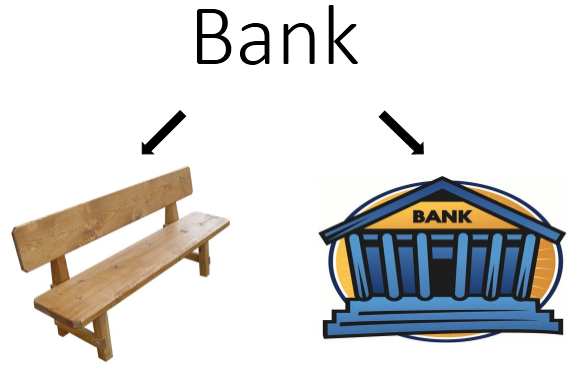
\includegraphics[scale=0.35]{disnomen}}
\end{figure}
}

\subsection{Disambiguierung in Dialogsystemen}
\frame{\frametitle{Disambiguierung in Dialogsystemen}
\begin{figure}[htbp]
	% minipage mit (Blind-)Text
	\begin{minipage}{0.5\textwidth} 
	\begin{itemize}
	\item "Rufe Peter an!"
	\newline
	\item System muss über Peter Meier und Peter Müller disambiguieren
	\newline
	\item unterschiedliche Disambiguierunsstrategien anwendbar
	\newline
	\end{itemize}
	\end{minipage}
	% Auffüllen des Zwischenraums
	\hfill
	% minipage mit Grafik
	\begin{minipage}{0.4\textwidth}
	% \textwidth bezieht sich nun auf die Minipage
	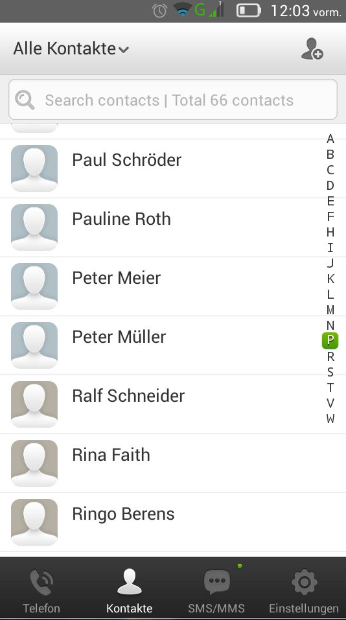
\includegraphics[scale=0.33]{peter}
	\label{Adressbuch} 
	\end{minipage}
% \caption{noch eine Caption}
\end{figure}
$\rightarrow$ 3 Disambiguierungstrategien untersucht
}
\subsection{1. Disambiguierungsstrategie}
\frame{\frametitle{1. Disambiguierungsstrategie: \\Aggregierte Auswahl ohne Pause}

\begin{itemize}
\item alle möglichen Interpretationen in einer Sprachausgabe 
\item keine Pause zwischen Interpretationen
\item auf Auswahl des Benutzers gewartet
\end{itemize}

\begin{table}
\begin{tabular}{l|l }
\textbf{Akteur} &	\textbf{Sprachausgabe}\\
\hline \hline
Benutzer & Rufe Peter an!\\
System & Meinst du Peter Müller oder Peter Meier?\\
Benutzer & Peter Müller.\\
System & Ok, ich werde Peter Müller jetzt anrufen.\\
\end{tabular}
%\caption{Interaktionsbeispiel \texttt{Aggregierte Auswahl ohne Pause}}
\end{table}


}
\subsection{2. Disambiguierungsstrategie}
\frame{\frametitle{2. Disambiguierungsstrategie: \\Aggregierte Auswahl mit Pause}
\begin{itemize}
\item alle möglichen Interpretationen in einer Sprachausgabe 
\item Pause und Nummerierung zwischen Interpretationen
\item auf Auswahl des Benutzers gewartet
\end{itemize}

\begin{table}
\begin{tabular}{l|l }
\textbf{Akteur} &	\textbf{Sprachausgabe}\\
\hline \hline
Benutzer & Rufe Peter an!\\
System & Meinst du [Pause] 1. Peter Müller\\
& [Pause] oder 2. Peter Meier?\\
Benutzer & Erstens \\
System & Ok, ich werde Peter Müller jetzt anrufen.\\
\end{tabular}
%\caption{Interaktionsbeispiel \texttt{Aggregierte Auswahl ohne Pause}}
\end{table} 
}
\subsection{3. Disambiguierungsstrategie}
\frame{\frametitle{3. Disambiguierungsstrategie: \\Sequentielle Auswahl}
\begin{itemize}
\item alle möglichen Interpretationen in einer separaten Sprachausgabe 
\item auf Zustimmung/Ablehnung des Benutzer gewartet
\end{itemize}

\begin{table}
\begin{tabular}{l|l }
\textbf{Akteur} &	\textbf{Sprachausgabe}\\
\hline \hline
Benutzer & Rufe Peter an!\\
System & Meinst du Peter Meier?\\
Benutzer & Nein.\\
System & Meinst du Peter Müller?\\
Benutzer & Ja.\\
System & Ok, ich werde Peter Müller jetzt anrufen.\\
\end{tabular}
%\caption{Interaktionsbeispiel \texttt{Aggregierte Auswahl ohne Pause}}
\end{table} 
}
\section{Versuch 1}
\subsection{Versuchsbeschreibung}
\frame{\frametitle{Kurzbeschreibung}
\begin{itemize}
\item Probanden fahren ein Rennspiel (hohe kognitive Belastung)
\item parellele Interaktion mit Dialogsystem                                                                                                                                                                                                                                                                                                                                                                                                                                                                                                                                                                                                                                                                                                                                                                                                                                                                                                                                                                                                                                                                                                                                                                                                                                                                               
\item alle Disambiguierungsstrategien pro Versuchsperson untersucht
\newline
\item Probanden interagieren ohne Rennspiel (geringe kognitive Belastung) 
\item eine Disambiguierungsstrategie zufällig getestet
\newline
\end{itemize}
$\rightarrow$ Disambiguierungsstrategien auf Effizienz und Beliebtheit untersucht \newline
$\rightarrow$ Ergebnisse mit und ohne Rennspiel werden miteinander verglichen 
}

\frame{\frametitle{Wizard-of-Oz}
\begin{itemize}
\item Die Existenz eines funktionierenden Systems wird vorgetäuscht
\newline
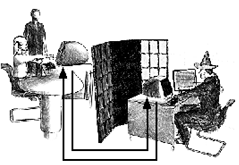
\includegraphics[scale=0.6]{woz}
\newline
\item Versuchspersonen wird der Eindruck verliehen, sie würde mit einem echten Dialogsystem interagieren
\item echtes Dialogsystem durch Versuchsleiter simuliert
\item Control Panel entwickelt, mit welchem Sprachausgaben ausgeben werden können
\end{itemize}
}

\frame{\frametitle{Testszenario}
\begin{itemize}
\item Versuchspersonen sollen erfolgreich per Sprachsteuerung einen Anruf aufbauen
\item insgesamt sollen vier Personen angerufen werden
\item nach Anrufinitialisierung wird simuliert, dass die Spracheingabe zu unspezifisch ist \newline $\rightarrow$ System stellt Rückfrage um zum Beispiel über mehrere mögliche Kontakte oder Telefonnummern zu disambiguieren
\item Nachfrage erfolgt in unterschiedlichen Strategien
\end{itemize}
\begin{block}{Beispiel} Benutzer: "Rufe Anke an" \newline System:\quad "Meinst du Anke Meier oder Schuhmacher?" \end{block} 

}

\frame{\frametitle{Testszenario}
\begin{figure}[htbp]
	% minipage mit (Blind-)Text
	\begin{minipage}{0.5\textwidth} 
		\begin{itemize}
			\item relevante Personenangaben (Slots) werden über ein Personenprofil angezeigt.
			\item pro Anruf werden jeweils 2 Slots abgefragt.
			\item die zufüllenden Slots unterscheiden sich pro anzurufenden Kontakt
			\item Rückfragen sind so generiert, dass der Slot an zweiter Stelle der zu füllende ist 
		\end{itemize}
	\end{minipage}
	\hfill
	\begin{minipage}{0.4\textwidth}
	\fbox{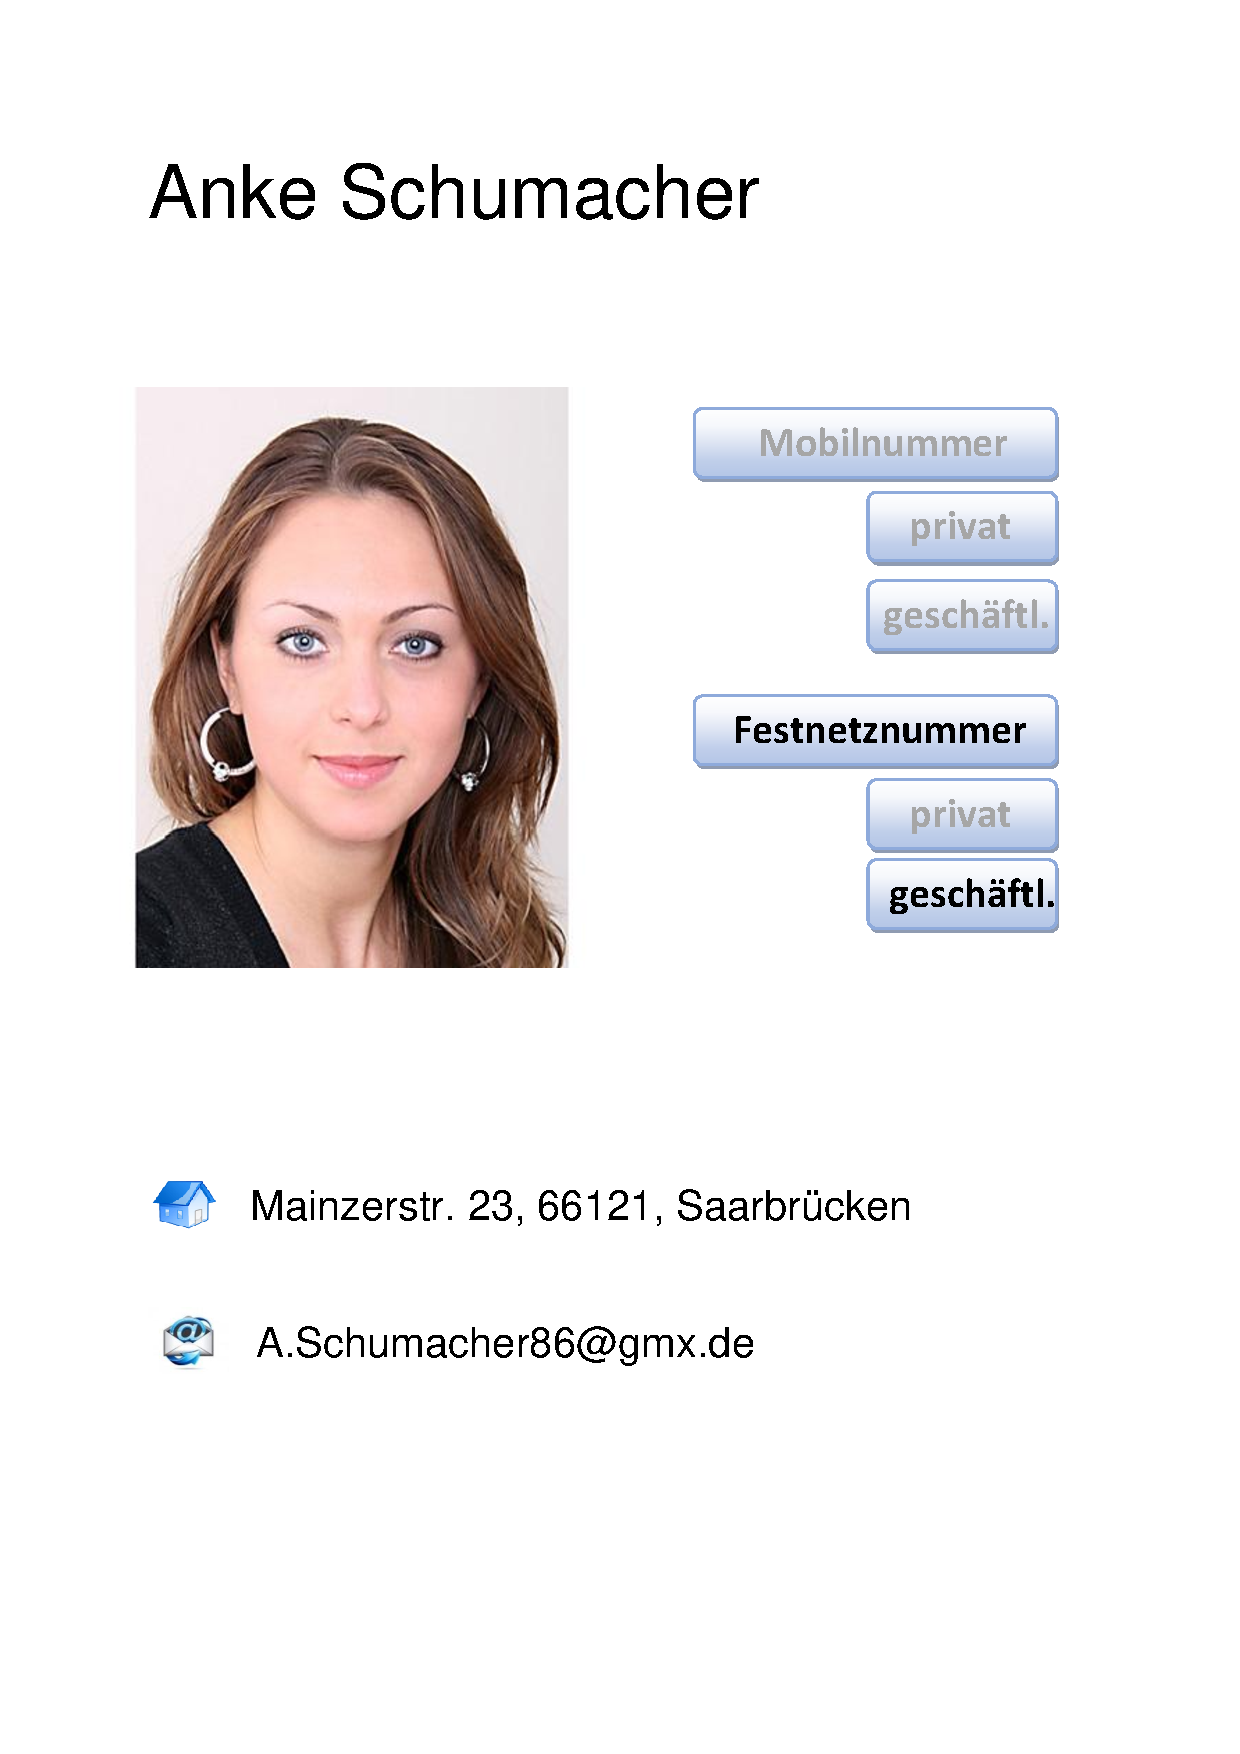
\includegraphics[scale=0.21]{Anke}}
	\label{Adressbuch} 
	\end{minipage}
% \caption{noch eine Caption}
\end{figure}
}

\frame{\frametitle{Versuchsaufbau}
\begin{itemize}
\item Versuchspersonen fahren ein Rennspiel. \newline $\rightarrow$ Fahrsimulation
\item Rennspiel: Need for Speed: Shift
\item Rennspiel wird mit Lenkrad inklusive Gas- und Bremspedal gespielt \newline $\rightarrow$ realitätsgetreues Gefühl
\item Es wird im Einzelrennen mit jeweils 5 Gegnern gespielt
\item Versuchspersonen sollen möglichst hohe Platzierung erreichen \newline $\rightarrow$ Anstrengung und Konzentration soll hohe kognitive Belastung verursachen
\end{itemize} 
}

\frame{\frametitle{Versuchsaufbau - Rennspiel}
\begin{figure}[h]
\caption{Need for Speed - Shift}
	%\centering
        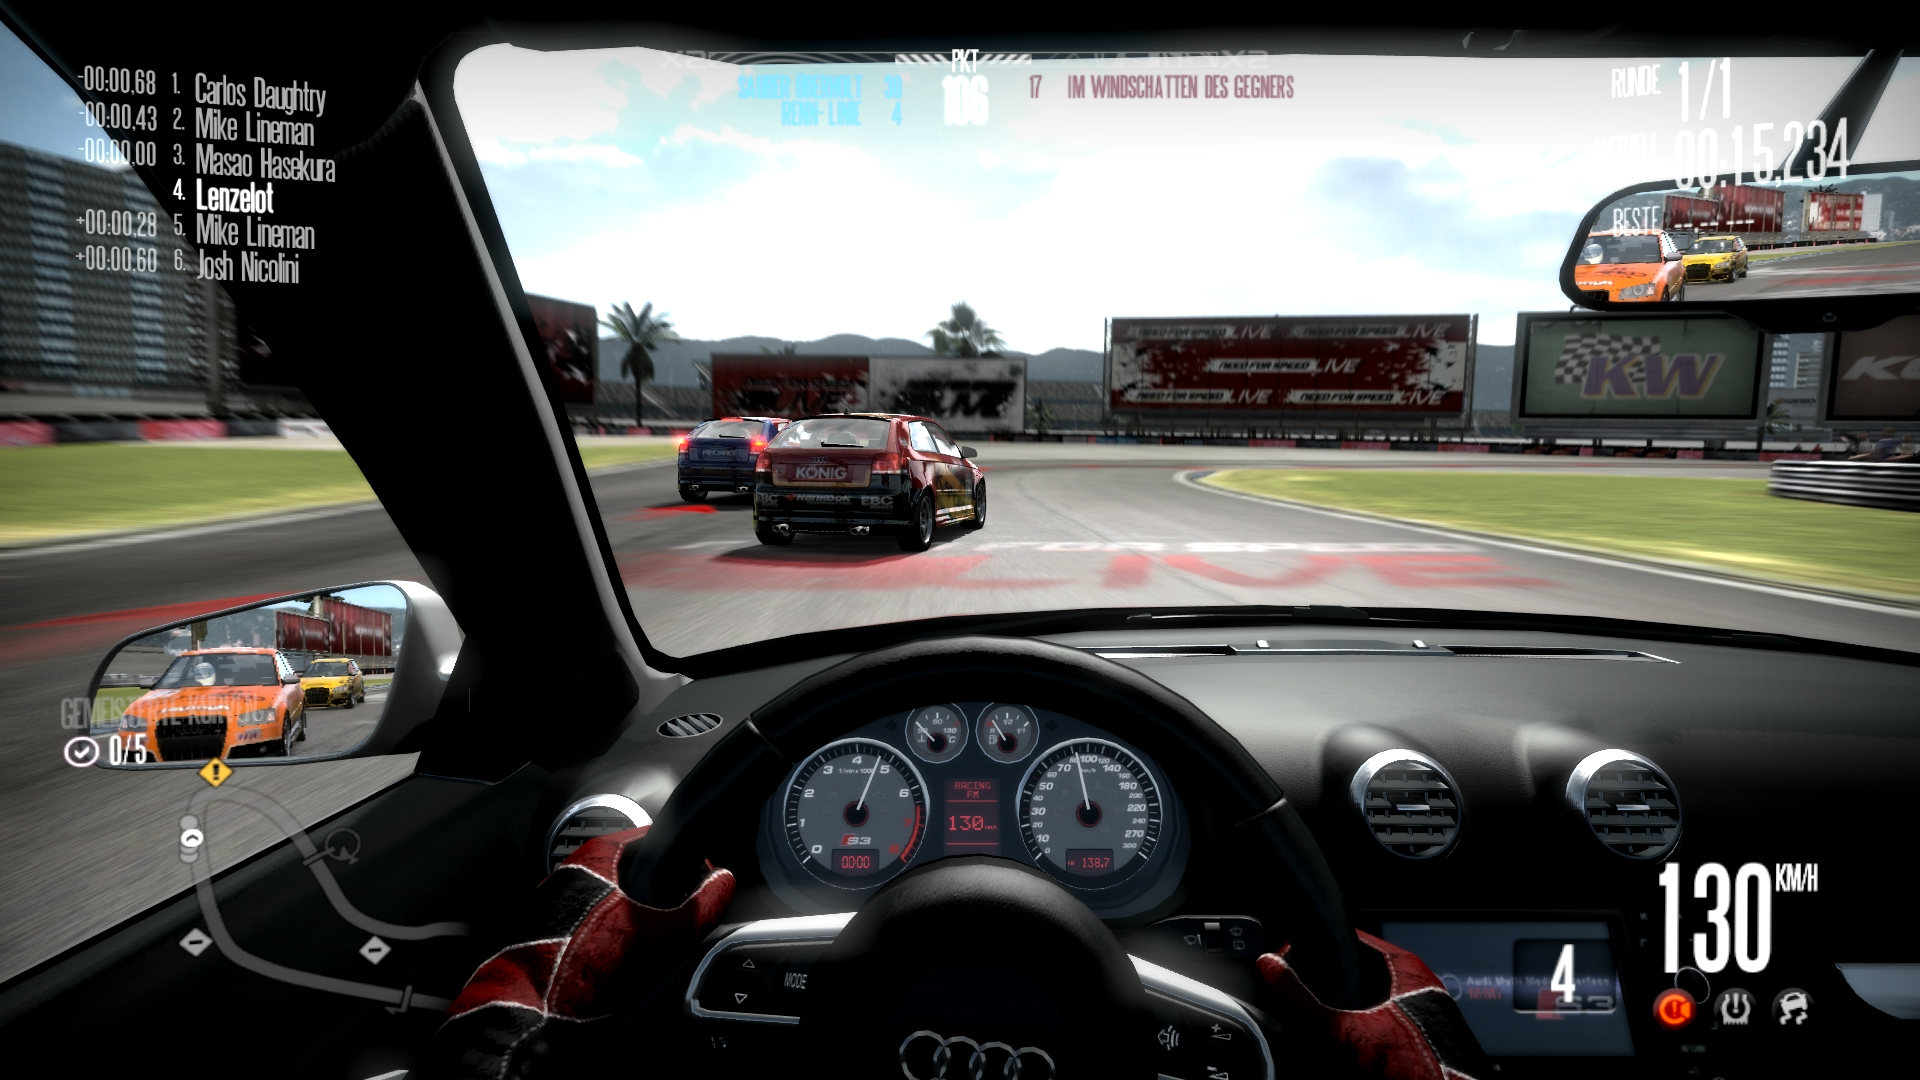
\includegraphics[scale=0.2]{nfs}
\end{figure}
}

\frame{\frametitle{Versuchsaufbau - Überblick}
\begin{table}
\begin{tabular}{l|l|l|l|l}
\textbf{Vorrunde}&\textbf{1. Runde}&\textbf{2. Runde} &\textbf{3. Runde} &\textbf{4. Runde}\\
\hline \hline
Rennspiel & Rennspiel & Rennspiel & Rennspiel &\\
 & Anruf Anke & Anruf Peter & Anruf Fritz & Anruf Kim \\
\end{tabular}
%\caption{Interaktionsbeispiel \texttt{Aggregierte Auswahl ohne Pause}}
\end{table}
\begin{itemize}
\item Vorrunde zum Einspielen
\item Runde 1-3: Rennspiel mit paralleler Systeminteraktion \newline $\rightarrow $ hohe kognitive Belastung
\item Runde 4: nur Systeminteraktion \newline $\rightarrow $ geringe kognitive Belastung
\end{itemize}
}

\frame{\frametitle{Versuchsdesign}
\begin{table}
\begin{tabular}{l|l|l|l}
\textbf{Aufteilung}&\textbf{Strecke 1}&\textbf{Strecke 2} &\textbf{Strecke 3}\\
\hline \hline
1. Gruppe & Strategie A & Strategie B & Strategie C \\
2. Gruppe & Strategie B & Strategie C & Strategie A\\
3. Gruppe  & Strategie C & Strategie A & Strategie B\\
4. Gruppe   & keine Strecke & keine Strecke & keine Strecke\\ 
\end{tabular}
%\caption{Interaktionsbeispiel \texttt{Aggregierte Auswahl ohne Pause}}
\end{table}
\begin{itemize}
\item 3 verschiedene Strecken, um Lerneffekt auszuschließen
\item jede Strecke mit unterschiedlicher Disambiguierungsstrategie
\item um Zeiten besser zu vergleichen: \newline $\rightarrow$ Disambiguierungsstrategien werden auf Strecken verteilt  \newline $\rightarrow$ Versuchspersonen werden in Gruppen (1-3) aufgeteilt
\item Die Strecken werden in gleicher Reihenfolge gefahren
\item Gruppe 4 führt das Testszenario mit zufälliger Strategie aus. 
\end{itemize}
}

\subsection{Control Panel}
\frame{\frametitle{Control Panel}
\begin{itemize}
\item entwickelt um ein laufendes Dialogsystem zu simulieren
\item verschiedene Sprachausgaben können per Mausklick abgespielt werden
\begin{figure}
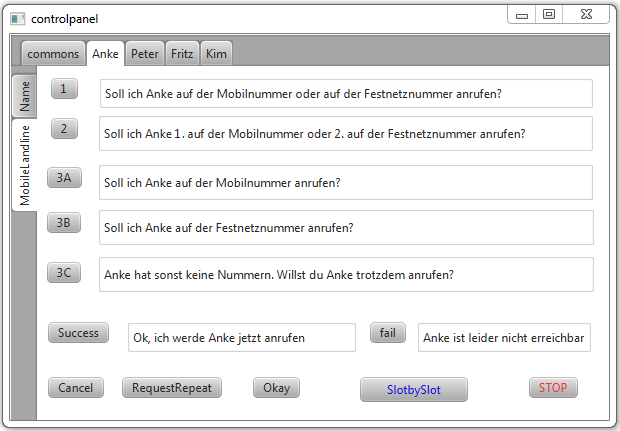
\includegraphics[scale=0.4]{controlpanel}
\end{figure}
\end{itemize}
}
\subsection{Versuchspersonen}
\frame{\frametitle{Versuchspersonen}
Versuchsablauf für eine Versuchsperson: \newline
\begin{enumerate}
\item Testrunde fahren
\item Fragebogen über eigene Person ausfüllen 
\item Strecke A fahren + Anke anrufen
\item Fragebogen über kognitive Belastung und Dialog ausfüllen 
\item Strecke B fahren + Peter anrufen
\item Fragebogen über kognitive Belastung und Dialog ausfüllen
\item Strecke C fahren + Fritz anrufen
\item Fragebogen über kognitive Belastung und Dialog ausfüllen 
\item Kim anrufen
\item Fragebogen über kognitive Belastung und Dialog ausfüllen 
\end{enumerate}
}

\frame{\frametitle{Versuchsperson - Fragebogen}
\begin{block}{Fragebogen über eigene Person} Informationen über Person für spätere Auswertung benötigt \end{block}
\begin{exampleblock}{Wie alt sind Sie?} Altereingabe \end{exampleblock}
\begin{table}
\begin{tabular}{l|l|l}
\textbf{18-29}&\textbf{30-41}&\textbf{42-53} \\
\hline \hline
58\% & 17\% & 25\% \\
\end{tabular}
%\caption{Interaktionsbeispiel \texttt{Aggregierte Auswahl ohne Pause}}
\end{table}
\begin{exampleblock}{Haben Sie Erfahrung mit Dialogsystemen?} 1: gar keine Erfahrung 6: viel Erfahrung \end{exampleblock}
\begin{table}
\begin{tabular}{l|l|l||l|l|l}
\textbf{1}&\textbf{2}&\textbf{3} & \textbf{4}&\textbf{5}&\textbf{6}  \\
\hline \hline
58\% & 8\% & 8\% & 8\% & 8\% & 8\%  
\end{tabular}
\end{table}
}

\frame{\frametitle{Versuchsperson - Fragebogen}
\begin{exampleblock}{Spielen Sie oft Rennspiele?} 1: sehr oft 6: nie  \end{exampleblock}
\begin{table}
\begin{tabular}{l|l|l||l|l|l}
\textbf{1}&\textbf{2}&\textbf{3} & \textbf{4}&\textbf{5}&\textbf{6}  \\
\hline \hline
0\% & 8\% & 8\% & 0\% & 56\% & 25\%  
\end{tabular}
\end{table}
\begin{exampleblock}{Wie technikaffin sind Sie?} 1: sehr technikaffin 6: gar nicht technikaffin \end{exampleblock}
\begin{table}
\begin{tabular}{l|l|l||l|l|l}
\textbf{1}&\textbf{2}&\textbf{3} & \textbf{4}&\textbf{5}&\textbf{6}  \\
\hline \hline
8\% & 17\% & 25\% & 33\% & 17\% & 0\%  
\end{tabular}
\end{table}
}

\frame{\frametitle{Versuchsperson - Fragebogen}
\begin{exampleblock}{Wie schwer fiel Ihnen die Einführungsrunde?} 1: sehr schwer 6: sehr einfach \end{exampleblock}
\begin{table}
\begin{tabular}{l|l|l||l|l|l}
\textbf{1}&\textbf{2}&\textbf{3} & \textbf{4}&\textbf{5}&\textbf{6}  \\

\hline \hline
8\% & 50\% & 0\% &8\% & 33\% & 0\%  
\end{tabular}
\end{table}
}

\subsection{Auswertung}
\frame{\frametitle{Auswertung}
Folgende Punkte werden ausgewertet
\newline
\begin{itemize}
\item Zeiten werden gemessen
	\begin{itemize}
		\item Rennzeiten
		\item Dialogzeiten
	\end{itemize}
\item Fragebögen ausgewertet
	\begin{itemize}
		\item Nasa-TLX
		\item Strategien
	\end{itemize}
\item Task Completion
\item Dialogverhalten
\end{itemize} 
}

\frame{\frametitle{Gemessene Zeiten - Rennzeiten}
\begin{block}{Rennzeiten}Beeinflusst eine Disambiguierungsstrategie das Rennverhalten? \end{block} 
\begin{table}
\begin{tabular}{l|l|l|l}
\textbf{Rennzeiten}&\textbf{Strategie 1}&\textbf{Strategie 2} &\textbf{Strategie 3}\\

\hline \hline
Strecke A & \textcolor{blue}{71,5 sek} & \textcolor{red}{93,0 sek} & 74,5 sek \\
Strecke B & \textcolor{blue}{68,8 sek} & 75,8 sek & \textcolor{red}{91,5 sek} \\
Strecke C & \textcolor{red} {74,5 sek} & \textcolor{blue}{58,4 sek} & 61,8 sek \\
\end{tabular}
\end{table} 
Werte könnten durch unbalancierte Gruppen entstehen.
\pause
\begin{table}
\begin{tabular}{l|l|l|l}
\textbf{Rennzeiten}&\textbf{Strategie 1}&\textbf{Strategie 2} &\textbf{Strategie 3}\\
\hline \hline
Durchschnitt & \textcolor{blue}{71,58 sek} & 75,71 sek & \textcolor{red}{75,92 sek} \\
\end{tabular}
\end{table}
Zeiten statistisch nicht relevant und daher nicht aussagekräftig. 
}

\frame{\frametitle{Gemessene Zeiten - Dialogzeiten}
\begin{block}{Dialogzeiten}Welche Strategie ermöglicht den kürzesten Dialog? \end{block} 
Nur die Zeiten von korrekt durchgeführten Dialogen bewertet.
\begin{table}
\begin{tabular}{l|l|l|l}
\textbf{Dialogzeiten}&\textbf{Strategie 1}&\textbf{Strategie 2} &\textbf{Strategie 3}\\

\hline \hline
Strecke A & \textcolor{blue}{15,3 sek} & \textcolor{red}{20,4 sek} & 20,3 sek \\
Strecke B & \textcolor{blue}{14,3 sek} & 20,1 sek & \textcolor{red}{22,1 sek} \\
Strecke C  & \textcolor{blue}{15,9 sek} & \textcolor{red}{21,0 sek} & 20,4 sek \\
\hdashline
ohne Strecke &  \textcolor{blue}{14,9 sek} & \textcolor{red}{18,8 sek} & 17,6 sek \\
\end{tabular}
\end{table} 
$\rightarrow$ Strategie 1 ermöglicht den kürzesten Dialog. 
}
\frame{\frametitle{Gemessene Zeiten - Dialogzeiten}
\begin{block}{Rennzeiten}Gibt es Unterschiede in den Dialogzeiten zwischen kognitiv hoch belasteten und kognitiv wenig belasteten Versuchspersonen? \end{block} 
\begin{table}
\begin{tabular}{l|l|l|l}
\textbf{Dialogzeiten}&\textbf{Strategie 1}&\textbf{Strategie 2} &\textbf{Strategie 3}\\

\hline \hline
Strecke A - C & \textcolor{red}{15,2 sek} & \textcolor{red}{20,5 sek} & \textcolor{red}{20,8 sek} \\
ohne Strecke &   \textcolor{blue}{14,9 sek} &  \textcolor{blue}{18,8 sek} &  \textcolor{blue}{17,6 sek} \\
\end{tabular}
\end{table} 
\begin{itemize}
\item kürzere Dialogzeiten ohne Rennspiel erreicht
\item Unterschiede nicht durch unterschiedliches Dialogverhalten erklärbar \newline
\end{itemize}
$\rightarrow$ bessere Reaktionszeit bei Dialoginteraktion ohne Rennspiel
}

\frame{\frametitle{Fragebogen - Nasa-TLX}
\begin{block}{Nasa-TLX} Bei welcher Stratgie wurde eine höhere Belastung empfunden? \newline \newline
Gibt es Unterschiede in der Belastung zwischen den Runden mit und ohne Rennspiel? \end{block}
}

\frame{\frametitle{Fragebogen - Nasa-TLX}
\begin{exampleblock}{Geistige Anfordung} 1: Gering 6: Hoch \end{exampleblock}

\begin{table}
\begin{tabular}{l|c|c|c}

%\textbf{Strategien}&\multicolumn{3}{c|}{\textbf{Ergebnisse bestimmter Runden}}\\
%&\textbf{1-4}&\textbf{1-3} &\textbf{4}\\
\textbf{Strategien}&\textbf{Runde 1-4}&\textbf{Runde 1-3} &\textbf{Runde 4}\\
	\hline \hline
Strategie 1 &  \textcolor{blue}{1,88} & \textcolor{blue}{2,08} & 1,25 \\
Strategie 2 & 2,06 & 2,42 & \textcolor{blue}{1,00}\\
Strategie 3 & \textcolor{red}{2,63} & \textcolor{red}{2,83} & \textcolor{red}{2,00} \\
\end{tabular}
\end{table}
\begin{itemize}
\item Strategie 1 geringe geistige Anforderung
\item Strategie 3 höchste geistige Anforderung
\newline
\item Runde 4 weniger anfordernd als Runden mit Rennspiel
\end{itemize}
}

\frame{\frametitle{Fragebogen - Nasa-TLX}
\begin{exampleblock}{Anstrengung} 1: Gering 6: Hoch \end{exampleblock}

\begin{table}
\begin{tabular}{l|c|c|c}

%\textbf{Strategien}&\multicolumn{3}{c|}{\textbf{Ergebnisse bestimmter Runden}}\\
%&\textbf{1-4}&\textbf{1-3} &\textbf{4}\\
\textbf{Strategien}&\textbf{Runde 1-4}&\textbf{Runde 1-3} &\textbf{Runde 4}\\
	\hline \hline
Strategie 1 & \textcolor{blue}{2,00} & \textcolor{blue}{2,25} & 1,25 \\
Strategie 2 & 2,13 & 2,55 & \textcolor{blue}{1,00} \\
Strategie 3 & \textcolor{red}{2,63} & \textcolor{red}{2,92} & \textcolor{red}{1,75}\\
\end{tabular}
\end{table}
\begin{itemize}
\item Strategie 1 geringeste Anstrengung
\item Strategie 3 höchste Anstrengung
\newline
\item Runde 4 weniger anstrengend als Runden mit Rennspiel
\end{itemize}
}

\frame{\frametitle{Fragebogen - Nasa-TLX}
Weitere Fragen
\begin{exampleblock}{Körperliche Anforderung} 1: Gering 6: Hoch \end{exampleblock}
\begin{exampleblock}{Zeitliche Anforderung} 1: Gering 6: Hoch \end{exampleblock}
\begin{exampleblock}{Leistung} 1: Gering 6: Hoch \end{exampleblock}
\begin{exampleblock}{Frustration} 1: Gering 6: Hoch \end{exampleblock}
}

\begin{comment}
\frame{\frametitle{Fragebogen - Nasa-TLX}
\begin{exampleblock}{Geistige Anfordung} 1: Gering 6: Hoch \end{exampleblock}

\begin{table}
\begin{tabular}{l|c|c|c}

%\textbf{Strategien}&\multicolumn{3}{c|}{\textbf{Ergebnisse bestimmter Runden}}\\
%&\textbf{1-4}&\textbf{1-3} &\textbf{4}\\
\textbf{Strategien}&\textbf{Runde 1-4}&\textbf{Runde 1-3} &\textbf{Runde 4}\\
	\hline \hline
Strategie 1 &  \textcolor{blue}{1,88} & \textcolor{blue}{2,08} & 1,25 \\
Strategie 2 & 2,06 & 2,42 & \textcolor{blue}{1,00}\\
Strategie 3 & \textcolor{red}{2,63} & \textcolor{red}{2,83} & \textcolor{red}{2,00} \\
\end{tabular}
\end{table}
Strategie 1 geringe geistige Anforderung, Strategie 3 höchste
\begin{exampleblock}{Haben Sie Erfahrung mit Dialogsystemen?} 1: gar keine Erfahrung 6: viel Erfahrung \end{exampleblock}
\begin{table}
\begin{tabular}{l|l|l||l|l|l}
\textbf{1}&\textbf{2}&\textbf{3} & \textbf{4}&\textbf{5}&\textbf{6}  \\
\hline \hline
58\% & 8\% & 8\% & 8\% & 8\% & 8\%  
\end{tabular}
\end{table}
}
\end{comment}


\frame{\frametitle{Fragebogen - Strategien}
\begin{block}{Strategien} Wie werden die Strategien von den Versuchspersonen bewertet? \end{block}

\begin{exampleblock}{Der Dialog lenkte mich stark vom Rennspiel ab} 1: kaum 6: stark \end{exampleblock}

\begin{table}
\begin{tabular}{l|c}

%\textbf{Strategien}&\multicolumn{3}{c|}{\textbf{Ergebnisse bestimmter Runden}}\\
%&\textbf{1-4}&\textbf{1-3} &\textbf{4}\\
\textbf{Strategien}&\textbf{Runde 1-3}\\
	\hline \hline
Strategie 1 &  \textcolor{blue}{2,25} \\
Strategie 2 & 2,58 \\
Strategie 3 & 2,58\\
\end{tabular}
\end{table}
$\rightarrow$ Strategie 1 lenkte am wenigsten vom Rennspiel ab
}

\frame{\frametitle{Fragebogen - Strategien}
\begin{exampleblock}{Wie gefiel Ihnen der Dialog insgesamt} 1: Gering 6: Hoch \end{exampleblock}

\begin{table}
\begin{tabular}{l|c|c|c}

%\textbf{Strategien}&\multicolumn{3}{c|}{\textbf{Ergebnisse bestimmter Runden}}\\
%&\textbf{1-4}&\textbf{1-3} &\textbf{4}\\
\textbf{Strategien}&\textbf{Runde 1-4}&\textbf{Runde 1-3} &\textbf{Runde 4}\\
	\hline \hline
Strategie 1 & \textcolor{blue}{1,94} & \textcolor{blue}{2,08} & \textcolor{blue}{1,50} \\
Strategie 2 & 2,50 & 2,67 & 2,00 \\
Strategie 3 & \textcolor{red}{2,57} & \textcolor{red}{2,75} & 2,00 \\
\end{tabular}
\end{table}
\begin{itemize}
\item Strategie 1 gefällt am besten
\item Strategie 3 gefällt am wenigsten
\end{itemize}
}

\frame{\frametitle{Fragebogen - Strategien}
\begin{exampleblock}{Fiel es Ihnen einfacher den Dialog ohne Rennspiel zu führen?} 1: viel einfacher 6: nicht einfacher \end{exampleblock}

\begin{table}
\begin{tabular}{l|c}

%\textbf{Strategien}&\multicolumn{3}{c|}{\textbf{Ergebnisse bestimmter Runden}}\\
%&\textbf{1-4}&\textbf{1-3} &\textbf{4}\\
\textbf{Strategien}&\textbf{Runde 4}\\
	\hline \hline
Strategie 1 & 2,00\\
Strategie 2 & 3,75 \\
Strategie 3 & 2,25\\
\end{tabular}
\end{table}
$\rightarrow$ der Dialog fiel im Durchschnitt ohne Rennspiel einfacher
}

\frame{\frametitle{Fragebogen - Strategien}
\begin{exampleblock}{Welcher Anruf gefiel Ihnen insgesamt am besten} Anruf bzw. Strategie auswählbar \end{exampleblock}

\begin{table}
\begin{tabular}{l|c}

%\textbf{Strategien}&\multicolumn{3}{c|}{\textbf{Ergebnisse bestimmter Runden}}\\
%&\textbf{1-4}&\textbf{1-3} &\textbf{4}\\
\textbf{Strategien}&\textbf{nach Versuch}\\
	\hline \hline
Strategie 1 & \textcolor{blue}{75,0\%}\\
Strategie 2 & 16,6\% \\
Strategie 3 & \textcolor{red}{8,3}\%\\
\end{tabular}
\end{table}
\begin{itemize}
\item Strategie 1 eindeutig am beliebtesten
\item Strategie 3 am unbeliebtesten
\end{itemize}
}



\frame{\frametitle{Fragebogen - Strategien}
Weitere Fragen
\begin{exampleblock}{Die Nachfragen erleichterten es mir, den Anruf korrekt aufzubauen} 1: erleichterte es 6: erschwerte es \end{exampleblock}
\begin{exampleblock}{Wussten Sie, wann das System Spracheingaben erwartete?} 1: immer 6: nicht immer \end{exampleblock}

\begin{itemize}
\item Strategie 1 am positivsten bewertet
\item Strategie 3 am negativsten bewertet
\end{itemize}
}

\frame{\frametitle{Task Completion}
\begin{block}{Task Completion (TC)} Welche Strategie ist am erfolgversprechendsten? \end{block}
\begin{itemize}
\item Die Task Completion wird für jeden Dialog wie folgt berechnet:
	\begin{itemize}
	\item 0 Punkte, wenn kein Slot richtig gefüllt wird
	\item 1 Punkt, wenn ein Slot richtig gefüllt wird
	\item 2 Punkte, wenn alle Slots richtig gefüllt werden
	\end{itemize}
\item für jede Strategie wird die durchschnittliche Task Completion bewertet
\end{itemize}
}

\frame{\frametitle{Task Completion}
%\begin{block}{Task Completion (TC)} Welche Strategie ist am erfolgversprechendsten? \end{block}

\begin{table}
\begin{tabular}{l|l|l|l}

\textbf{Strategien}&\textbf{Runde 1-4}&\textbf{Runde 1-3} &\textbf{Runde 4}\\
	\hline \hline
1. Strategie & 1,75 & 1,92 & 1,50  \\
2. Strategie & \textcolor{blue}{1,94} & 1,92 & 2,00  \\
3. Strategie & \textcolor{red}{1,63} & 1,50 & 2,00  \\
\hdashline
alle Strategien & & \textcolor{red}{1,78} & \textcolor{blue}{1,83} \\ 
\end{tabular}
\end{table}

\begin{itemize}
\item Strategie 2 am erfolgreichsten
\item Strategie 3 am erfolgreichsten 
\item Runde ohne Rennspiel erfolgreicher als Runden mit Rennspiel\newline \newline $\rightarrow$ Unterschied gering: Mehr Werte benötigt für aussagekräftiges Ergebnis
\newline
\end{itemize}

}


\frame{\frametitle{Auswertung - Zusammenfassung}
\begin{itemize}
\item \textbf{kürzeste Rennzeit}: nicht aussagekräftig
\item \textbf{kürzeste Dialogzeit}: Strategie 1
\item Ergebnis \textbf{Nasa-TLX} Fragebogen:
	\begin{itemize}
		\item Strategie 1 am unbelastetsten
		\item Runde ohne Rennspiel weniger belastend als Runde mit
	\end{itemize}
\item Ergebnis \textbf{Fragebogen} Strategie:
	\begin{itemize}
		\item Strategie 1 am positivsten bewertet
		\item Dialog fiel im Durchschnitt ohne Rennspiel einfacher
	\end{itemize}
\item \textbf{Task Completion} 
	\begin{itemize}
		\item Strategie 2 > Strategie 1 > Strategie 3 (geringer Unterschied)
		\item Dialog ohne Rennspiel erfolgreicher als Dialog ohne REnnspiel
	\end{itemize}
\end{itemize}
$\Rightarrow$ \textcolor{blue}{Strategie 1} am Effizientesten und Beliebtesten
}



\section{Versuch 2}
\subsection{Versuchsbeschreibung}
\frame{\frametitle{Vorahnung}
\textsl{"The wise man avoids evil by anticipating it" (Publilius Syrus)}
\newline

Vorahnung ist lebenswichtig
\begin{itemize}
\item kein Halten von gef\"ahrlichen Tieren als Haustiere
\item keine Spazierg\"ange bei Gewitter                                                                                                                                                                                                                                                                                                                                                                                                                                                                                                                                                                                                                                                                                                                                                                                                                                                                                                                                                                                                                                                                                                                                                                                                                                                                               
\item Reflexe aus\"uben
\end{itemize} 
}
\begin{comment}
\subsection{Versuchsaufbau}
\frame{\frametitle{Vorahnung}
\textsl{"The wise man avoids evil by anticipating it" (Publilius Syrus)}
\newline

Vorahnung ist lebenswichtig
\begin{itemize}
\item kein Halten von gef\"ahrlichen Tieren als Haustiere
\item keine Spazierg\"ange bei Gewitter                                                                                                                                                                                                                                                                                                                                                                                                                                                                                                                                                                                                                                                                                                                                                                                                                                                                                                                                                                                                                                                                                                                                                                                                                                                                               
\item Reflexe aus\"uben
\end{itemize} 
}
\subsection{Versuchsdesign}
\frame{\frametitle{Vorahnung}
\textsl{"The wise man avoids evil by anticipating it" (Publilius Syrus)}
\newline

Vorahnung ist lebenswichtig
\begin{itemize}
\item kein Halten von gef\"ahrlichen Tieren als Haustiere
\item keine Spazierg\"ange bei Gewitter                                                                                                                                                                                                                                                                                                                                                                                                                                                                                                                                                                                                                                                                                                                                                                                                                                                                                                                                                                                                                                                                                                                                                                                                                                                                               
\item Reflexe aus\"uben
\end{itemize} 
}
\end{comment}
\subsection{Control Panel}
\frame{\frametitle{Vorahnung}
\textsl{"The wise man avoids evil by anticipating it" (Publilius Syrus)}
\newline

Vorahnung ist lebenswichtig
\begin{itemize}
\item kein Halten von gef\"ahrlichen Tieren als Haustiere
\item keine Spazierg\"ange bei Gewitter                                                                                                                                                                                                                                                                                                                                                                                                                                                                                                                                                                                                                                                                                                                                                                                                                                                                                                                                                                                                                                                                                                                                                                                                                                                                               
\item Reflexe aus\"uben
\end{itemize} 
}
\subsection{Versuchspersonen}
\frame{\frametitle{Vorahnung}
\textsl{"The wise man avoids evil by anticipating it" (Publilius Syrus)}
\newline

Vorahnung ist lebenswichtig
\begin{itemize}
\item kein Halten von gef\"ahrlichen Tieren als Haustiere
\item keine Spazierg\"ange bei Gewitter                                                                                                                                                                                                                                                                                                                                                                                                                                                                                                                                                                                                                                                                                                                                                                                                                                                                                                                                                                                                                                                                                                                                                                                                                                                                               
\item Reflexe aus\"uben
\end{itemize} 
}

\subsection{Auswertung}
\frame{\frametitle{Vorahnung}
\textsl{"The wise man avoids evil by anticipating it" (Publilius Syrus)}
\newline

Vorahnung ist lebenswichtig
\begin{itemize}
\item kein Halten von gef\"ahrlichen Tieren als Haustiere
\item keine Spazierg\"ange bei Gewitter                                                                                                                                                                                                                                                                                                                                                                                                                                                                                                                                                                                                                                                                                                                                                                                                                                                                                                                                                                                                                                                                                                                                                                                                                                                                               
\item Reflexe aus\"uben
\end{itemize} 
}
\subsection{Resultat}
\frame{\frametitle{Vorahnung}
\textsl{"The wise man avoids evil by anticipating it" (Publilius Syrus)}
\newline

Vorahnung ist lebenswichtig
\begin{itemize}
\item kein Halten von gef\"ahrlichen Tieren als Haustiere
\item keine Spazierg\"ange bei Gewitter                                                                                                                                                                                                                                                                                                                                                                                                                                                                                                                                                                                                                                                                                                                                                                                                                                                                                                                                                                                                                                                                                                                                                                                                                                                                               
\item Reflexe aus\"uben
\end{itemize} 
}

\section{Ergebnisse}
\frame{\frametitle{Vorahnung}
\textsl{"The wise man avoids evil by anticipating it" (Publilius Syrus)}
\newline

Vorahnung ist lebenswichtig
\begin{itemize}
\item kein Halten von gef\"ahrlichen Tieren als Haustiere
\item keine Spazierg\"ange bei Gewitter                                                                                                                                                                                                                                                                                                                                                                                                                                                                                                                                                                                                                                                                                                                                                                                                                                                                                                                                                                                                                                                                                                                                                                                                                                                                               
\item Reflexe aus\"uben
\end{itemize} 
}
\section{Fazit}
\frame{\frametitle{Vorahnung}
\textsl{"The wise man avoids evil by anticipating it" (Publilius Syrus)}
\newline

Vorahnung ist lebenswichtig
\begin{itemize}
\item kein Halten von gef\"ahrlichen Tieren als Haustiere
\item keine Spazierg\"ange bei Gewitter                                                                                                                                                                                                                                                                                                                                                                                                                                                                                                                                                                                                                                                                                                                                                                                                                                                                                                                                                                                                                                                                                                                                                                                                                                                                               
\item Reflexe aus\"uben
\end{itemize} 
}

\end{document}

